\chapter{Realisierung}
In diesem Kapitel wird die Realisierung des Entwicklungssystems
beschrieben. <\ldots>
\section{Konfiguration des Carambola}
OpenWRT bietet mit dem Programm \gls{uci} eine Anwendung, Einstellungen
zentralisiert zu verwalten. Über das \gls{uci}-System lassen sich unter anderem
Ethernet, WLAN, DHCP und SSH-Server konfigurieren. Die einzelnen
Einstellungsdateien liegen alle im Verzeichnis \listinlsh{/etc/config/} und
können mittels des Tools modifiziert werden.

Nach Systemstart werden außerdem alle Dateien im Ordner
\listinlsh{/etc/uci-defaults/} eingelesen, ausgeführt und anschließend gelöscht.
Dies erlaubt es Softwarepaketen, Einstellungen am System vorzunehmen. Werden
diese Softwarepakete bereits in die Firmware integriert, entspricht dies einer
Art Vorkonfiguration des Systems.
\subsection{WLAN und Netzwerkkonfiguration}
Da die Netzwerkkonfiguration von OpenWRT vollständig durch die
\gls{uci}-Konfigurationsdateien abgewickelt wird, muss auch \gls{uci} genutzt
werden, wenn das Netzwerk vorkonfiguriert werden soll.

\gls{uci} bietet mit \listinlsh{uci batch} explizit einen Befehl an, um
umfangreiche Einstellungsändeurngen vorzunehmen. Hierfür werden die einzelnen
Befehle mittels \emph{Here document} übergeben.
\begin{lstlisting}[language=sh]
uci batch <<-EOF_network
	...
	commit network
	EOF_network
\end{lstlisting}

 \begin{definition}[Here document]
Ein \emph{Here document} ermöglicht es, einem Unix-Befehl mehrere, durch
Zeilenumbrüche getrennte, Befehle zu übergeben.
\end{definition}

\subsection{Aktivierung des UART}\label{subs:aktuart}
Der Mikrochip\cite{RA01} des Carambolas besitzt zwei \glspl{uart}. Einer dieser
\glspl{uart} wird für die Serielle Konsole verwendet und somit kann der zweite
Anschluss für die Datenschnittstelle des Entwicklungssystems verwendet werden.
Da die Pins des Carambolas für den zweiten \gls{uart} standardmäßig auf
\gls{gpio}-Betrieb eingestellt sind, müssen diese erst umgestellt werden.

Hierzu muss das Tool \texttt{io} installiert und mittels 
\listinlsh{io 0x10000060 0x01} ausgeführt werden. Dies setzt im Speicher des
Mikrocontrollers das Flag, den \gls{uart} zu aktivieren. Dieser Vorgang muss
nach jedem Systemstart erfolgen und kann durch die, bei jedem Systemstart
aufgerufene, \listinlsh{/etc/rc.local} erfolgen.

Zusätzlich muss verhindert werden, dass auf diesem \gls{uart} eine Linuxterminal
betrieben wird. Hierzu muss die Datei \listinlsh{/etc/inittab} modifiziert
werden.

Diese beiden Änderungen werden wie folgt ebenso mittels des Skripts in
\listinlsh{/etc/uci-defaults} durchgeführt.
\begin{lstlisting}[language=sh]
sed -i '/exit 0/ i\io 0x10000060 0x01' /etc/rc.local
sed -i '/ttyS0/ s/^/# /' /etc/inittab
\end{lstlisting}

\section{OpenOCD}
Für OpenOCD existiert keine Portierung in die Paketverwaltung von OpenWRT. Es
muss also ein Makefile erstellt werden, das die Einbindung ermöglicht. Der
grundlegende Aufbau solcher Makefiles ist im Wiki von OpenWRT
festgelegt\cite{OWRT}.

Um OpenOCD kompilieren zu können, müssen zuerst die Voraussetzungen festgestellt
werden. Da ein auf dem FT2232-Chip basierender \gls{jtag}-Adapter mit
USB-Anschluss eingesetzt werden soll, müssen laut \texttt{README} von OpenOCD
sowohl libftdi als auch libusb installiert sein. Diese Pakete stehen für OpenWRT
bereits zur Verfügung und müssen im Makefile als Abhängigkeiten definiert
werden. Dies geschieht mit dem Befehl \listinlsh{DEPENDS:=+libftdi +libusb}.

Der Quellcode von OpenOCD wird durch das Makefile in der Version 0.6.1 von
Sourceforge selbstständig heruntergeladen, über MD5 verifiziert und entpackt.

Vor dem Kompilierungsvorgang müssen noch die an \listinlsh{./configure}
zu übergebenden Argumente festgelegt werden. Der verwendete Adapter erfordert
hier die Option \listinlsh{--enable-ft2232_libftdi}.

<\ldots>
<Vorkonfiguration von OpenWRT/OpenOCD>
\section{Server - FreeJTAG}
Der "`FreeJTAG"' genannte Server des Entwicklungssystems wird auf dem Carambola
installiert, als Serveranwendung bei jedem Systemstart gestartet und leitet die
gesammelten Daten an jeden verbundenen Client weiter.

Für die Funktion dieser Software müssen zu Beginn einige Einstellungen
festgelegt werden. Hierzu zählen die Parameter der \gls{uart}-Verbindung
(Baudrate, Parität, Stopp-Bit) und der Netzwerkport.

\subsection{Bibliotheken und Abhängigkeiten}
Als Bibliotheken kommen bei FreeJTAG vor allem Teile der Boost Bibliothek zum
Einsatz. Diese dienen der asynchronen Netzwerkkommunikation (Boost ASIO), dem
hierfür nötigen Einsatz von Threads (Boost Thread), der Verwaltung der
Zeitstempel (Boost Chrono) und dem Speichern von Programmeinstellungen (Boost
Program\_Options).

Außerdem hängt FreeJTAG von dem Paket "`io"' ab, da dieses für die Aktivierung
des \gls{uart}, wie in \autoref{subs:aktuart} beschrieben, zuständig ist und
installiert werden muss. Die in \autoref{subs:aktuart} beschriebene Skriptdatei
ist ebenso in diesem Paket enthalten. 

Durch die Installation dieser Anwendung wird das Carambola also komplett für den
Einsatz als Entwicklungssystem konfiguriert.

\subsection{Strukturierung der Serversoftware}
\begin{figure}[!ht]
\centering
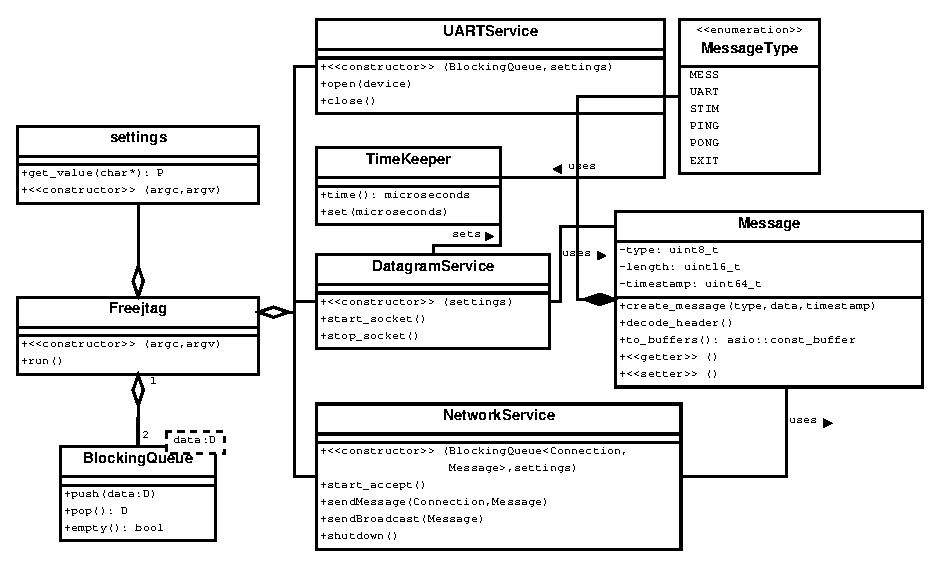
\includegraphics[width=\textwidth]{server.eps}
\caption{Grober Aufbau der Serveranwendung}{Diese Abbildung verdeutlicht den
Aufbau der Serveranwendung (FreeJTAG). Hierbei wurden Details zu Gunsten der
Übersichtlichkeit ausgelassen.}
\label{fig:server}
\end{figure}
\autoref{fig:server} stellt eine grobe Übersicht über den Aufbau der
Serveranwendung dar. Hierbei wurden Details wie weitere Klassen und
zusätzliche Aggregationen zwischen den einzelnen Elementen zugunsten einer
besseren Übersicht ausgelassen.

Die Hauptanwendung \texttt{Freejtag} dient als "`Bindeglied"' zwischen den
einzelnen Bestandteilen der Software. Die genaueren Abläufe hierzu sollen in
\autoref{subs:abl} erläutert werden.

Weiterhin besteht die Serversoftware aus einer Klasse
\texttt{NetworkService} zur Übertragung der Nutzdaten, \texttt{DatagramService}
um die Zeitsynchronisation über UDP zu managen und \texttt{UARTService} für den
Empfang der Daten vom Zielsystem.

Die Klasse \texttt{Message} dient zum Parsen der Netzwerkdaten und wird somit
sowohl vom TCP- als auch vom UDP-Dienst verwendet.

Da die Zeitstempel synchronisiert werden sollen, wurde die Klasse
\texttt{TimeKeeper} erstellt. Sie dient dem Setzen der Zeitdifferenz und der
Abfrage des aktuellen Zeitstempels unter Berücksichtigung der gespeicherten
Differenz.

Die Hilfsklasse \texttt{BlockingQueue} wird als Schnittstelle zwischen dem
Hauptprogramm und dem \texttt{UARTService} sowie zwischen dem Hauptprogramm
und dem \texttt{NetworkService} eingesetzt. Sie ist nötig, da jeder dieser
Dienste in einem anderen Thread läuft und der Datenaustausch aus diesem Grund
synchronisiert werden muss.

\subsection{ASIO - Asynchrone Netzwerkkommunikation}\label{subs:asio}
Für die Netzwerkkommunikation kommt die Bibliothek ASIO des Boost-Projektes zum
Einsatz. Sie erleichtert die Nutzung asynchroner Netzwerkvorgänge.

Hierbei läuft die Netzwerkkommunikation wie folgt ab:

<\ldots>
\subsection{Programmablauf}\label{subs:abl}
Die Anwendung wird zuerst initialisiert und anschließend ausgeführt. Dies
erfolgt durch folgenden Ablauf.
\begin{lstlisting}[language=C++]
int main(int argc, char* argv[]) {
    freejtag::Freejtag *prog;
    prog = new freejtag::Freejtag(argc, argv);
    int res = prog->run();
    delete prog;
    return res;
}
\end{lstlisting}
Bei Erstellung des \texttt{Freejtag}-Objektes werden zuerst aus
\listinlsh{/etc/freejtag.cfg} und die per Parameter (und in diesem Fall
Kommandozeile) übergebenen Einstellungen eingelesen.
Das Einlesen dieser Werte erfolgt unter Nutzung der
\emph{Boost.Program\_options}-Bibliothek. Tritt hierbei ein Fehler auf, wird das
Programm mit einer Fehlermeldung beendet.

Intern werden die über das Netzwerk zu versendenden und empfangenen Nachrichten
mittels \texttt{shared\_ptr}(Smart Pointer) von \texttt{Message}-Objekten
verwendet. Es muss nun eine \\\texttt{BlockingQueue} initialisiert werden, die
die über den TCP-Port empfangenen Nachrichten verwaltet. Da bei
TCP-Sendevorgängen direkt die in \autoref{subs:asio} erläuterten Abläufe
verwendet werden, ist eine weitere \texttt{BlockingQueue} zur Synchronisierung
hierfür nicht notwendig.

Da es möglich sein soll mehrere Verbindungen (Siehe auch \autoref{subs:best}) zu
verwalten, muss in der \texttt{BlockingQueue} zusammen mit der \texttt{Message}
auch immer die Verbindung von der sie erhalten wurde gespeichert werden.

Eine zweite \texttt{BlockingQueue} dient zur Erfassung der über UART gesammelten
Daten mit zugehörigen Zeitstempeln. 

Nun werden sowohl \texttt{NetworkService} als auch \texttt{DatagramService}
initialisiert.

Der \texttt{NetworkService} erhält hierfür die vorher erstellte
\texttt{BlockingQueue}(den Buffer), legt das Protokoll auf TCP fest und
öffnet den in den Einstellungen spezifizierten Port. Der Ablauf des
\texttt{DatagramService} verläuft analog mit dem Unterschied, dass für die über
diesen Dienst erfolgende Zeitsynchronisation kein Zugriff auf den
Nachrichten-Buffer nötig ist.

Anschließend werden zwei Threads gestartet, die für die Abwicklung der, durch
den Empfang von UART- oder Netzwerkdaten angestoßenen, Vorgänge zuständig
ist. Hierfür warten die Threads mittels \listinlcpp{UARTMessage msg =
input_uart_.pop();} beziehungsweise \newline\listinlcpp{MessageDatagram msgd =
input_network_.pop();} auf die Ankunft neuer Daten in ihrere zugehörigen
\texttt{BlockingQueue}. Dies schließt die Initialisierung ab.

Da sowohl UART-Empfang wie auch TCP-Sendevorgänge asynchron
abgewickelt werden, werden hierfür keine weiteren Threads benötigt (Siehe
\autoref{subs:asio}). 

Nun muss nun \listinlcpp{Freejtag::run();} aufgerufen werden, um den Start der
Anwendung zu vollziehen. Dies startet ein asynchrones Accept auf dem Socket des
Netzwerkmoduls, so dass es nun möglich ist, eine Verbindung zum Server
herzustellen. Der \gls{uart}-Anschluss wird auf dem angegebenen Gerät geöffnet
und mit den eingestellten Parametern konfiguriert.

<\ldots>



\begin{itemize}
  \item Integration in OpenWRT
  \item Bibliotheken
  \item Aufbau der Anwendung
  \item ASIO
  \item \ldots
\end{itemize}
\section{Client - The Kraken}
\begin{itemize}
  \item Funktionalität - Verbinden, Trennen, Synchronisieren, Erfassen
  \item Sortierung der Daten - Treemap
  \item MVC, maven und andere Spielereien
\end{itemize}
\section{Deployment}
\begin{itemize}
  \item Scripting von OpenOCD
  \item Einbindung in Eclipse
\end{itemize}
\section{Datenanalyse (FreeJTAG)}
<\ldots>